\section{AI-Assisted Authoring Workflow}
\label{sec:authoring-workflow}

\begin{figure}
    \centering
    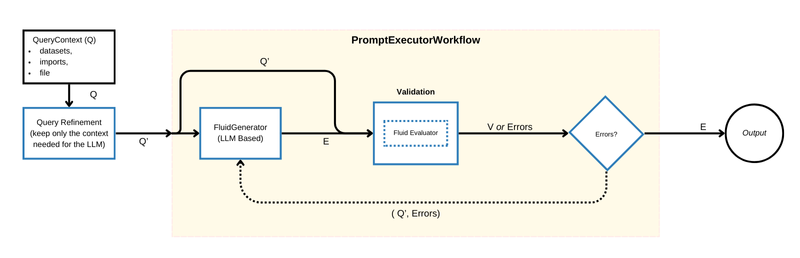
\includegraphics[width=0.95\linewidth]{fig/authoring-assistant-architecture.png}
    \caption{AI-assisted authoring workflow}
\end{figure}

\subsection{Editor Loop}
Design of main loop that would be integrated into an IDE. The configuration (state) that is being maintained
is a \kw{Paragraph} the user is authoring in Fluid. Consists of a sequence of text fragments, some of which
are uninterpreted (plain literals), the remainder have underlying expressions linking the text to raw or derived
data.

Workflow:
\begin{enumerate}
\item User selects (a substring of) one of the literal text fragments, indicating they want to link it in this
way
\item Authoring tool generates expression which is either:
  \begin{enumerate}
  \item computes the selected text (e.g.~``greater than'' might be computed by comparing two numbers)
  \item becomes the formal meaning of the selected text (e.g. the text ``carbon intensity of methane
emissions'' can be understood in a specific context as referring to the numerical value ``34 gCO2eq/kWh''
  \end{enumerate}
\item Some kind of validation step, including both automated validation (e.g. checking for runtime errors) and
user validation; if validation fails, goto (2)
\item Partition code into additional definitions and expression; add definitions to main source file, and
incorporate expression into \kw{Paragraph}
\item Goto (1) with updated editor state
\end{enumerate}

\subsection{Turning validation errors into improved prompts}
E.g.:
\begin{enumerate}
\item Turn ``Definition not found'' into prompt to generate definition?
\end{enumerate}

\subsection{IDE integration}

Could then be integrated into desktop IDE like VSCode or online IDE like CodeMirror. Might make a good
internship project, but could also be out-of-scope for this paper.

\subsection{Other potential enhancements}

We could also think about using an LLM in a couple of other complementary ways:
\begin{itemize}
\item identifying text fragments which might be linked;
\item validating generated expressions (perhaps by proposing test cases)
\end{itemize}
